%!TEX root = main.tex
\clearpage
\section{Conclusion}

\subsection{Global vision}

In table \ref{tab:operators_status}, it is possible to view (marked green), the operators that were implemented in the first semester of this dissertation. As it can be seen, I have implemented five of the thirteen operators that João Durães specified. The first operator that I have implemented with success was the \ac{mifs} one, and as the operators \ac{mia} and \ac{mieb} are similar and have some constraints in common, I also implemented them.

% \clearpage
% \begin{table}[ht]
% \begin{tabular}{c}
% 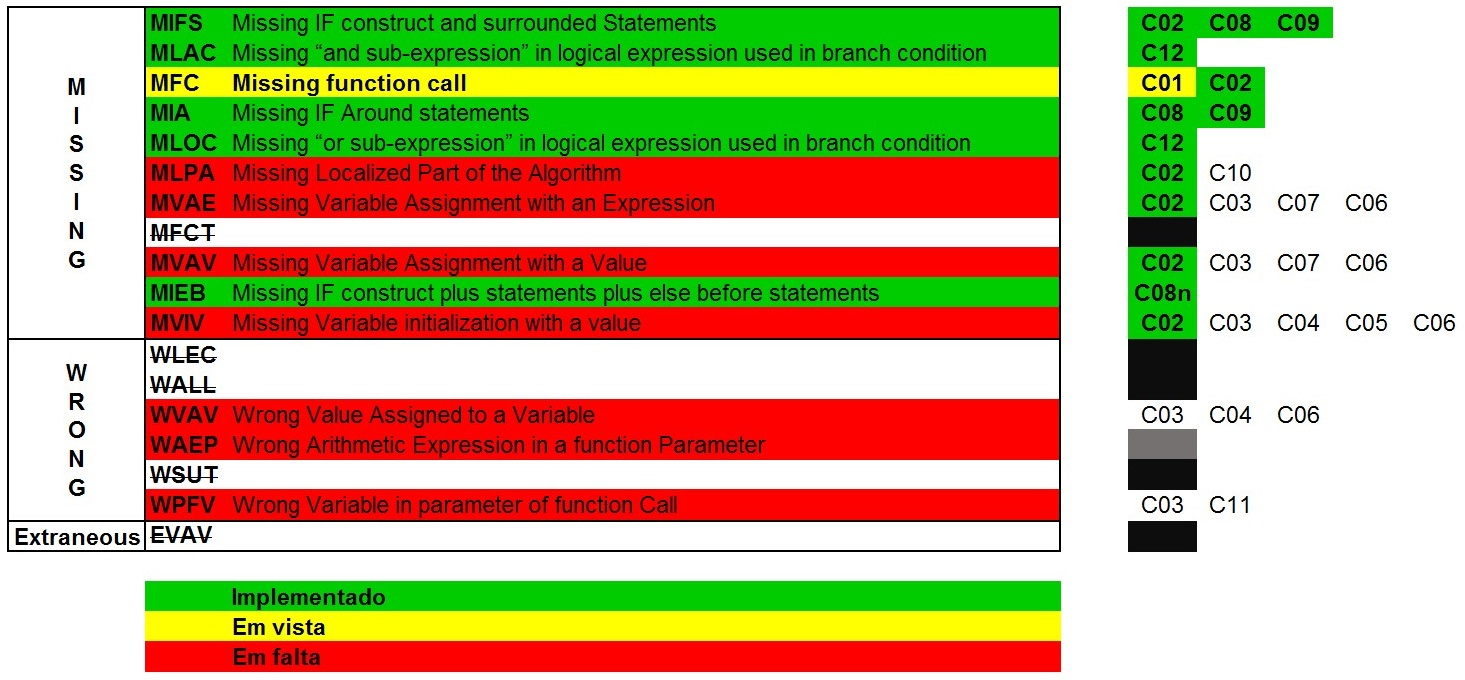
\includegraphics[width=1.1\textwidth]{img/operators_status.jpg}
% \end{tabular}
% \caption{\small \sl State of the operators and its constraints.\label{tab:operators_status}}
% \end{table}


\begin{table}[!ht]
\begin{tabular}{|l|p{12cm}|}
\hline
\textbf{Fault Type}		& \multicolumn{1}{c|}{\textbf{Description}}		\\ \hline \hline
MFC        				& \Acl{mfc}  									\\ \hline
\green{MIA}        		& \green{\Acl{mia}} 							\\ \hline
\green{MIEB}       		& \green{\Acl{mieb}} 							\\ \hline
\green{MIFS}       		& \green{\Acl{mifs}} 							\\ \hline
\green{MLAC}       		& \green{\Acl{mlac}} 							\\ \hline
\green{MLOC}       		& \green{\Acl{mloc}} 							\\ \hline
MLPA       				& \Acl{mlpa} 									\\ \hline
MVAE       				& \Acl{mvae} 									\\ \hline
MVAV       				& \Acl{mvav} 									\\ \hline
MVIV       				& \Acl{mviv} 									\\ \hline
WAEP       				& \Acl{waep} 									\\ \hline
WPFV       				& \Acl{wpfv} 									\\ \hline
WVAV       				& \Acl{wvav} 									\\ \hline
\end{tabular}
\caption{\small \sl State of the operators.\label{tab:operators_status}}
\end{table}

In table \ref{tab:constraints_status}, is also possible to check that I have implemented three of the eleven constraints related to the thirteen operators, represented in \green{green}.

\begin{table}[!ht]
\centering
\begin{tabular}{|c|p{12cm}|}
\hline
\textbf{Constraints}            & \multicolumn{1}{c|}{\textbf{Description}}                                     \\ \hline \hline
\textbf{C01}         & \Acl{c01} \\ \hline
\green{\textbf{C02}} & \green{\Acl{c02}} \\ \hline
\textbf{C03}         & \Acl{c03} \\ \hline
\textbf{C04}         & \Acl{c04} \\ \hline
\textbf{C05}         & \Acl{c05} \\ \hline
\textbf{C06}         & \Acl{c06} \\ \hline
\textbf{C07}         & \Acl{c07} \\ \hline
\green{\textbf{C08}} & \green{\Acl{c08}} \\ \hline
\green{\textbf{C09}} & \green{\Acl{c09}} \\ \hline
\textbf{C10}         & \Acl{c10} \\ \hline
\textbf{C11}         & \Acl{c11} \\ \hline
\end{tabular}
\caption{\small \sl State of the constraints.\label{tab:constraints_status}}
\end{table}

\begin{table}[!ht]
\centering
\begin{tabular}{|c|p{12cm}|}
\hline
\textbf{Constraints}            & \multicolumn{1}{c|}{\textbf{Description}}                                     \\ \hline \hline
\green{\textbf{C08n}}         & \green{\Acl{c08n}} \\ \hline
\green{\textbf{C12}}          & \green{\Acl{c12}} \\ \hline
\end{tabular}
\caption{\small \sl State of the other constraints.\label{tab:otherConstraints_status}}
\end{table}

% \iftoggle{long}{\red{version number}}
\break
Below, in figure \ref{tab:version}, it can be seen the version numbering system of this fault injector. The ``b'' letter states that there are two constraints implemented which are not specified by João Durães. For instance, if I had implement three constraints, then it will be ``c'', and so on. The current version of the injector also has five operators and three constraints implemented, from those specified by João Durães. When the version numbering reaches 0.13.11 then the injector will be in version number one.

\begin{figure}[!ht]
\begin{center}
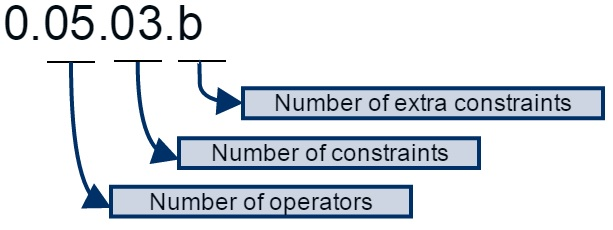
\includegraphics[width=0.6\textwidth]{version.jpg}
\caption{\small \sl Version number.\label{tab:version}}
\end{center}
\end{figure}

\clearpage
\subsection{Future work and experiments}

In the future, I have planned to implement the remaining operators and constraints. I will use regression testing to verify that when I code one new operator or constraint I do not mess with the operators and constraints previously implemented.
In addition to this, I will add to the fault injector a user interface, in order to make it more user-friendly, and a name.

Furthermore, in the next semester, I will study the hypervisor and I will implement some scenarios to evaluate the behavior of the cloud with and without faults.



% \textit{``The purpose of regression testing is to ensure that changes made to software, such as adding new features or modifying existing features, have not adversely affected features of the software that should not change. Regression testing is usually performed by running some, or all, of the test cases created to test modifications in previous versions of the software.''}
% \red{From version to version, I use a regression testing to test the fault injector to guarantee that application doesn't regarded.}

\iftoggle{long}{\orange{Mais do que “future work” é necessário um plano para o segundo semestre, relativamente detalhado.}}


% \iftoggle{long}{\orange{Globalmente há várias coisas que não estão suficientemente bem explicadas:}}


\iftoggle{long}{\orange{- exatamente quais são as características novas da cloud, que devem ser avaliadas por injeção de falhas (podemos conversar sobre isto)}}


% \iftoggle{long}{\orange{- qual a razão para se desenvolver algo novo, quando a ferramenta do Natella já faz muito (lembro-me que colecionámos muitos argumentos que estão anotados)}}


% \iftoggle{long}{\orange{- como é que se vai dar uso ao que está implementado? far-se-ão experiências, os resultados serão classificados e analisados certamente}}


% \iftoggle{long}{\orange{- o estado da arte deveria ponderar os prós e os contras de todas as técnicas para injeção de falhas de software (binário, instrumentação, source code, runtime, etc.)}}


% \iftoggle{long}{\orange{- o texto deve ser clarificado, mas essencialmente é no plano das ideias que muitas vezes está pouco claro: por que razão se está a fazer isto?}}


\iftoggle{long}{\orange{- quais são as alternativas? como é feito? exatamente o que é feito}}


\iftoggle{long}{\red{Regression Testing}}


\iftoggle{long}{\red{System testing}}


\iftoggle{long}{\red{Unit tests}}


\iftoggle{long}{\red{Performance analyses}}

% \subsubsection{Experiments}

% In the next semester, additionally of the conclusion of the fault injector, I'll inject faults in the cloud.
In figure \ref{fig:test1}, it can be seen two environments where the first and second experiments will be done, under normal conditions (without faults) and with faults, respectively. An application will be selected, as shown in the figure as ``App''. This application will run in a normal environment and it will be measured the runtime and the result of the execution, for later comparison with the results obtained in other scenarios.

\begin{figure}[!ht]
\begin{center}
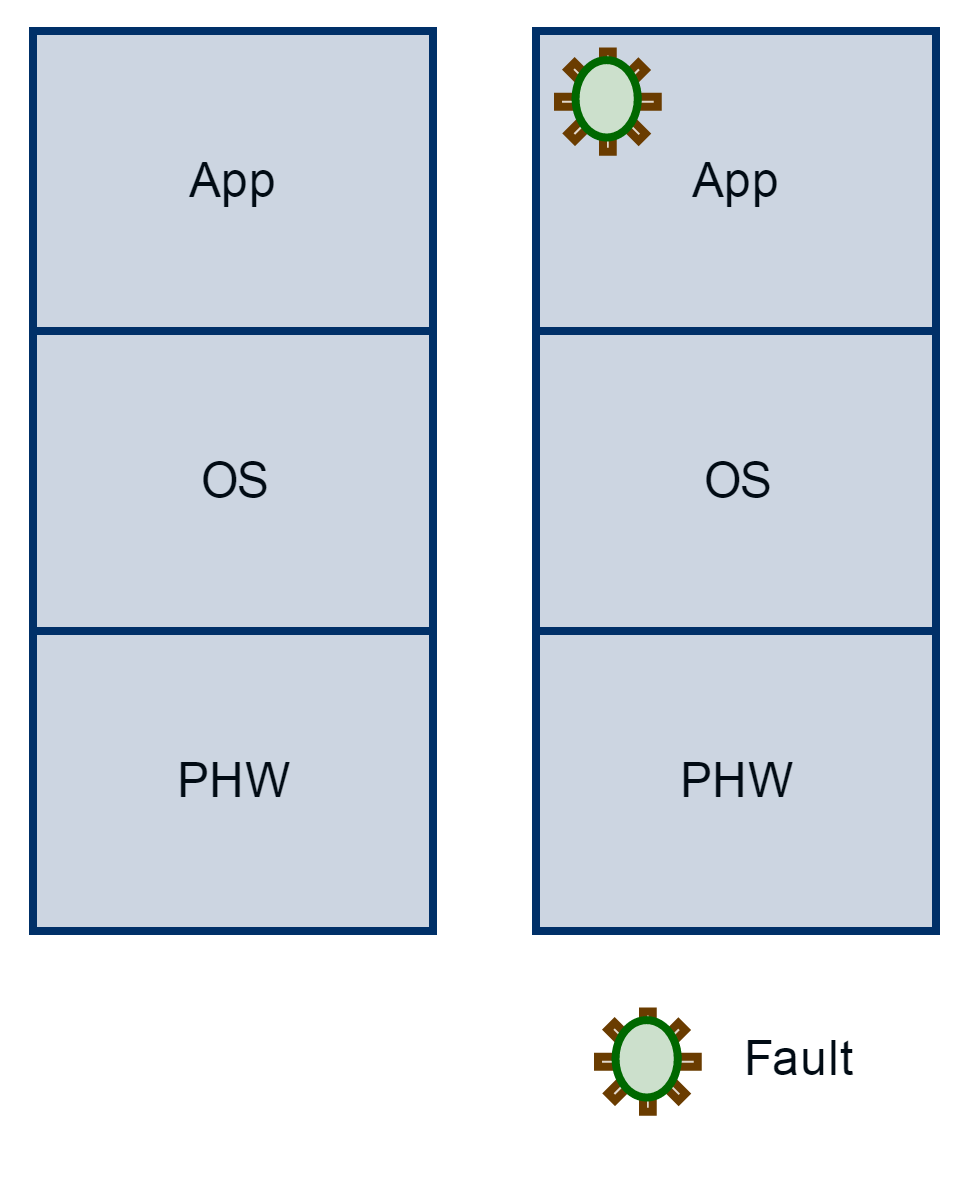
\includegraphics[width=0.4\textwidth]{test1.png}
\caption{\small \sl First and second experiments.\label{fig:test1}}
\end{center}
\end{figure}

The scenario represented in the right side of figure \ref{fig:test1} is similar to the one in the left side, with the slight  difference that the latter one has a fault injected into the ``App''. Depending on the type of fault injected into the ``App'', it will have different behaviors, which will be assessed by the \emph{CRASH Scale}.

% \begin{figure}[!ht]
% \begin{center}
% \includegraphics[width=0.2\textwidth]{test2.png}
% \caption{\small \sl Second experiment.\label{fig:test2}}
% \end{center}
% \end{figure}

Below, in figure \ref{fig:test3}, it is represented the third experiment with an Native Hypervisor. The goal of this scenario is to evaluate whether through fault injection in one of the virtual machines, the others are affected. It will also try to evaluate if the virtual machine without faults exhibits the same behavior when running side by side with a virtual machine that has an ``App'' with faults and without faults.

% \begin{figure}[!ht]
% \begin{center}
% 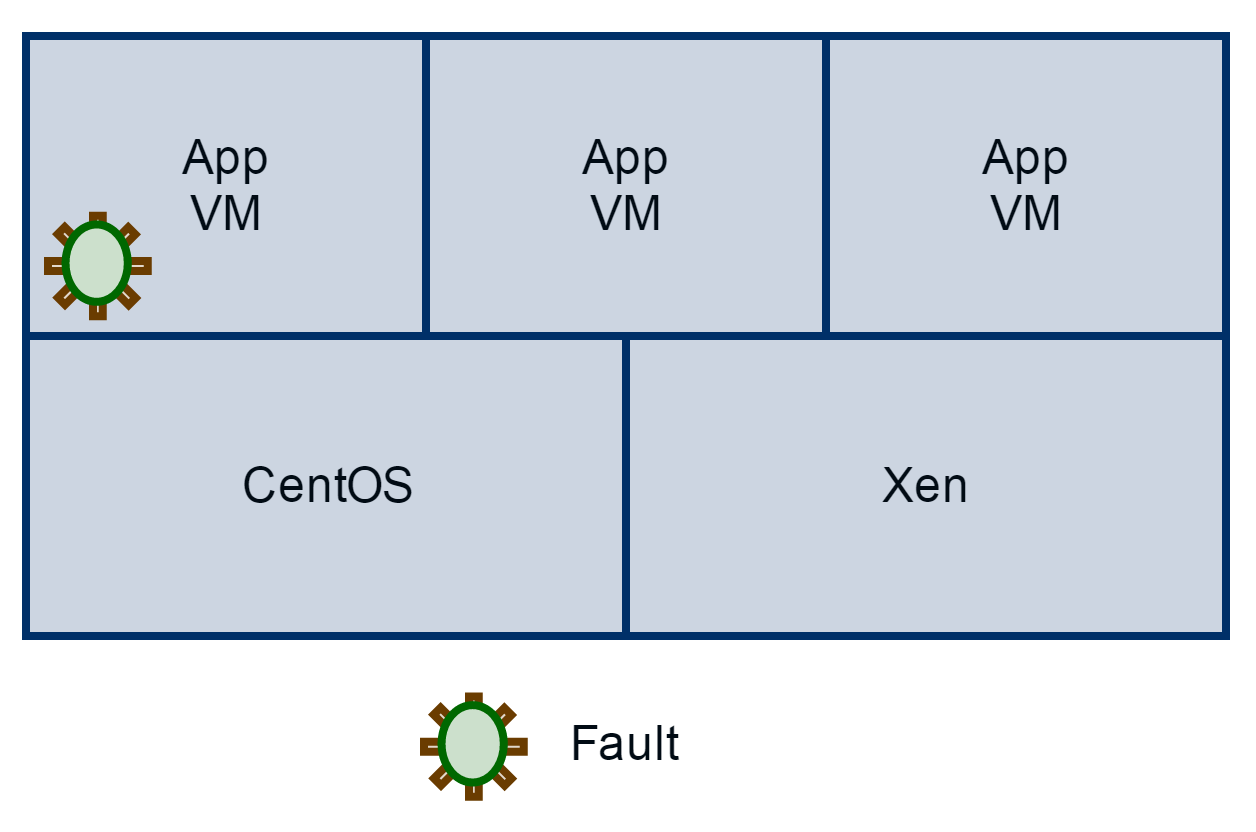
\includegraphics[width=0.5\textwidth]{test3.png}
% \caption{\small \sl Third experiment.\label{fig:test3}}
% \end{center}
% \end{figure}


\begin{figure}[!ht]
\begin{center}
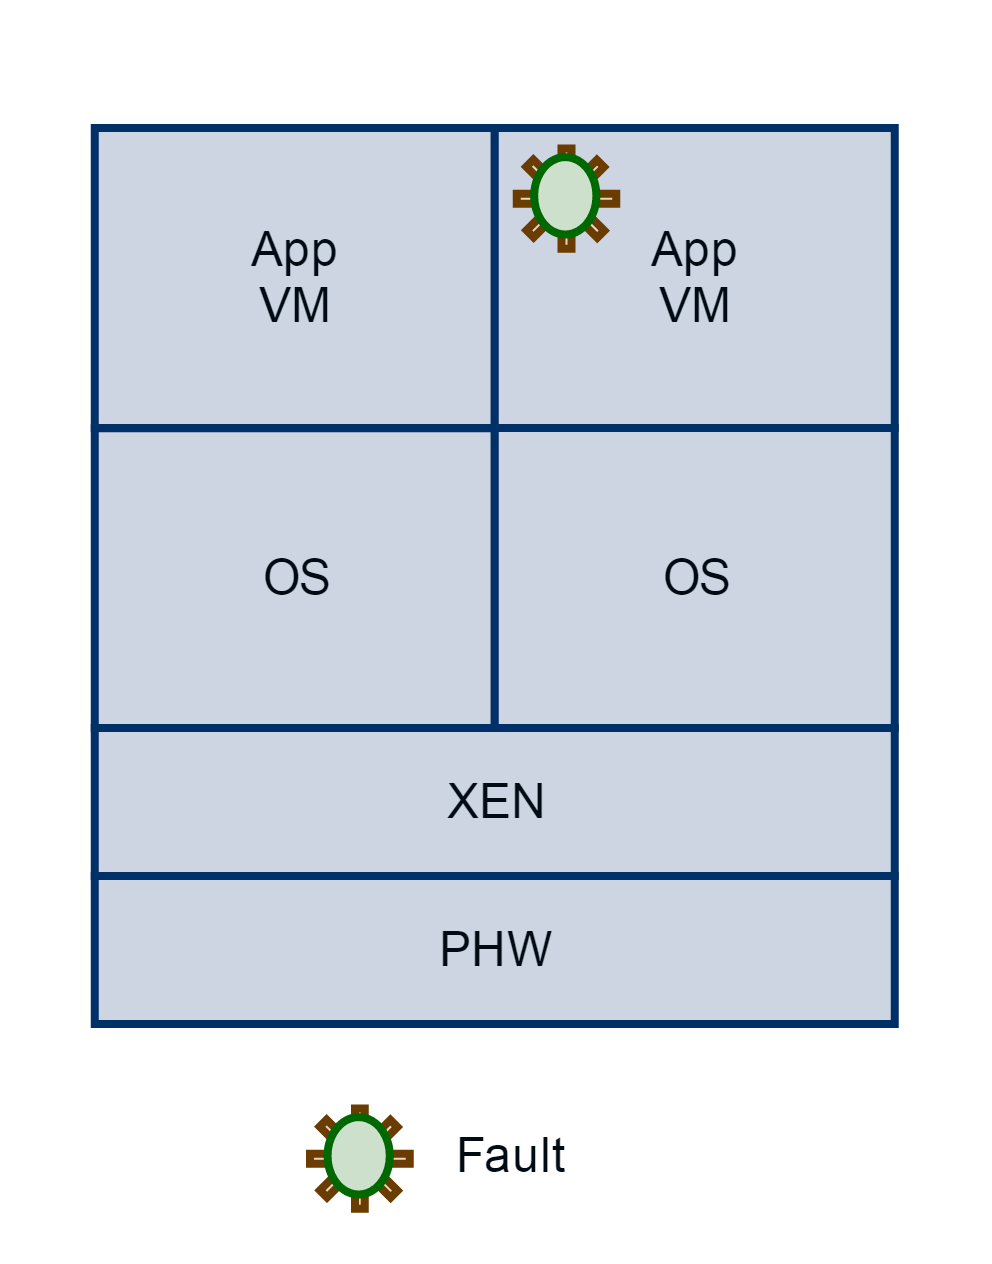
\includegraphics[width=0.4\textwidth]{test4.png}
\caption{\small \sl Third experiment.\label{fig:test3}}
\end{center}
\end{figure}

% \red{The same applications that João Durães has collected information?}
% \begin{itemize}
% 	\item MinGW, Last Update: 2015-06-08
% 	\item ScummVM, Last Update: 2015-05-17
% 	\item CDEX, Last Update: 2015-04-24
% 	\item FireBird, Last Update: 2015-04-15
% 	\item Joe, Last Update: 2015-03-22
% 	\item FreeCiv, Last Update: 2015-03-14
% 	\item GAIM or Pidgin, Last Update: 2015-01-07
% 	\item BASH, Last Update: 2013-12-10
% 	\item ZSNES, Last Update: 2013-05-07
% 	\item VIM, Last Update: 2013-04-25
% 	\item pdftohtml, Last Update: 2013-04-24
% 	%\item LKERNEL
% \end{itemize}
